\documentclass[tikz,convert]{standalone}

\usetikzlibrary{decorations.pathreplacing}

\begin{document}
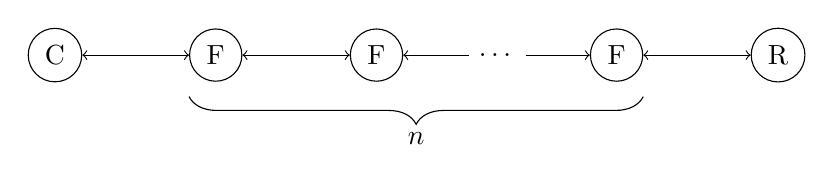
\begin{tikzpicture}
  
  \node[draw, shape=circle] (c) {C};
  \node[draw, shape=circle, right of=c, right=20pt] (f1) {F};
  \node[draw, shape=circle, right of=f1, right=20pt] (f2) {F};
  \node[right of=f2, right=5pt] (ellipsis) {\ldots};
  \node[draw, shape=circle, right of=ellipsis, right=5pt] (fn) {F};
  \node[draw, shape=circle, right of=fn, right=20pt] (r) {R};
  
  \path[draw, <->] (c) to (f1);
  \path[draw, <->] (f1) to (f2);
  \path[draw, <-] (f2) to (ellipsis);
  \path[draw, ->] (ellipsis) to (fn);
  \path[draw, <->] (fn) to (r);

  \draw[decorate, decoration={brace, mirror, amplitude=10pt}]
  ([yshift=-15pt] f1.west) -- ([yshift=-15pt] fn.east)
  node [midway, yshift=-15pt] {$n$};
  
\end{tikzpicture}
\end{document}
